\chapter{Stacked bar plots}

In this chapter, we will work towards creating the bar plot below. We
will take you from a basic stacked bar plot and explain all the
customisations we add to the code step-by-step.

\begin{center}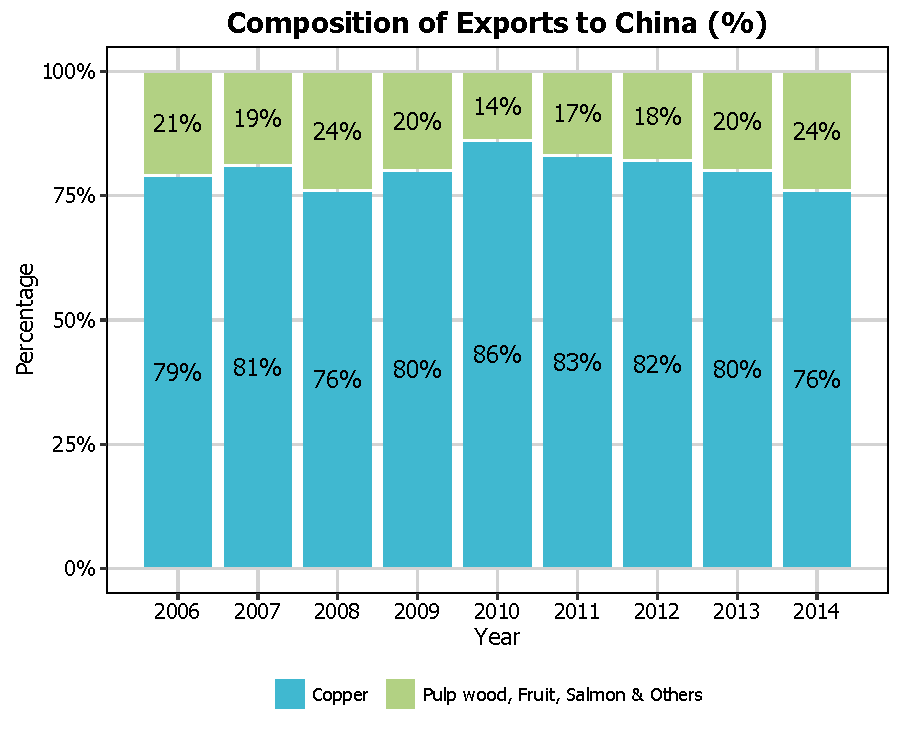
\includegraphics[width=0.6\linewidth]{4_Stacked_Bar_pdf/stacked_finalresult-1} \end{center}

\section{Basic graph}\label{basic-graph}

In order to initialise a plot we tell ggplot that \texttt{charts.data}
is our data, and specify the variables on each axis. We then instruct
ggplot to render this as a stacked bar plot by adding the
\texttt{geom\_bar} command.

We will use the same data as in Chapter \ref{chapter1}.

The first thing to do is load in the data and libraries, as below:

\begin{Shaded}
\begin{Highlighting}[]
\KeywordTok{library}\NormalTok{(ggplot2)}
\KeywordTok{library}\NormalTok{(ggthemes)}
\KeywordTok{library}\NormalTok{(extrafont)}
\KeywordTok{library}\NormalTok{(plyr)}
\KeywordTok{library}\NormalTok{(scales)}

\NormalTok{charts.data <-}\StringTok{ }\KeywordTok{read.csv}\NormalTok{(}\StringTok{"copper-data-for-chapter.csv"}\NormalTok{)}
\end{Highlighting}
\end{Shaded}

\begin{Shaded}
\begin{Highlighting}[]
\NormalTok{p4 <-}\StringTok{ }\KeywordTok{ggplot}\NormalTok{() +}\StringTok{ }\KeywordTok{geom_bar}\NormalTok{(}\KeywordTok{aes}\NormalTok{(}\DataTypeTok{y =} \NormalTok{percentage, }\DataTypeTok{x =} \NormalTok{year, }\DataTypeTok{fill =} \NormalTok{product), }
  \DataTypeTok{data =} \NormalTok{charts.data, }\DataTypeTok{stat=}\StringTok{"identity"}\NormalTok{)}
\NormalTok{p4}
\end{Highlighting}
\end{Shaded}

\begin{center}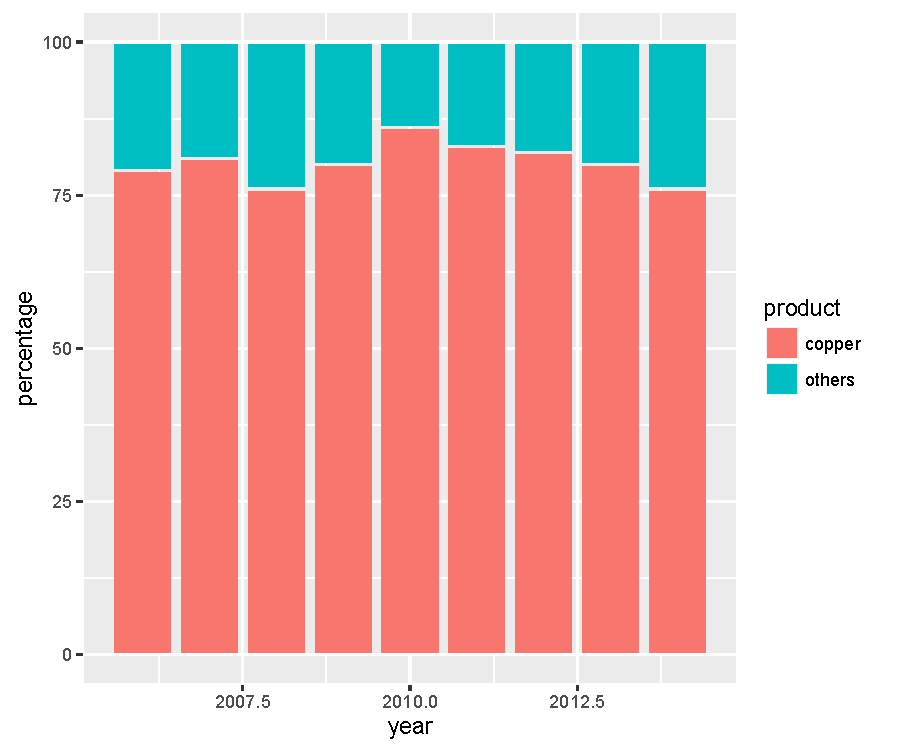
\includegraphics[width=0.6\linewidth]{4_Stacked_Bar_pdf/stacked_1-1} \end{center}

\section{Adding data labels}\label{adding-data-labels}

To label the bars according to some variable in the data, we add the
\texttt{label} argument to the \texttt{ggplot(aes())} option. In this
case, we have labelled the bars with numbers from the \texttt{export}
variable.

\begin{Shaded}
\begin{Highlighting}[]
\NormalTok{p4 <-}\StringTok{ }\NormalTok{p4 +}\StringTok{ }\KeywordTok{geom_text}\NormalTok{(}\DataTypeTok{data=}\NormalTok{charts.data, }\KeywordTok{aes}\NormalTok{(}\DataTypeTok{x =} \NormalTok{year, }\DataTypeTok{y =} \NormalTok{percentage, }
  \DataTypeTok{label =} \KeywordTok{paste0}\NormalTok{(percentage,}\StringTok{"%"}\NormalTok{)), }\DataTypeTok{size=}\DecValTok{4}\NormalTok{)}
\NormalTok{p4}
\end{Highlighting}
\end{Shaded}

\begin{center}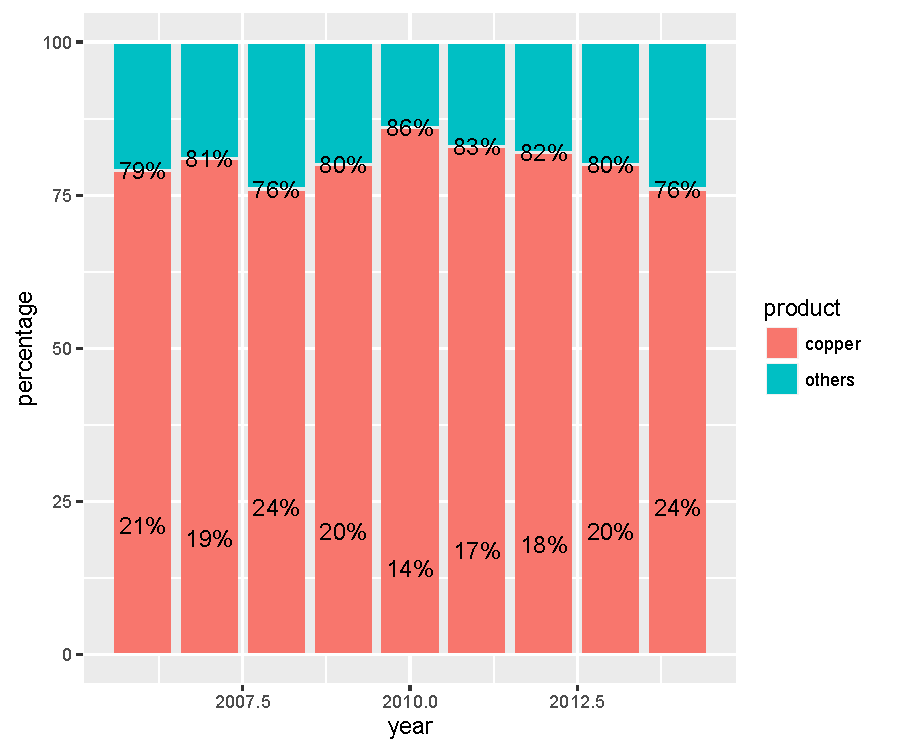
\includegraphics[width=0.6\linewidth]{4_Stacked_Bar_pdf/stacked_2-1} \end{center}

\section{Adjusting data labels
position}\label{adjusting-data-labels-position}

To adjust the position of the data labels from the default placement, we
use the \texttt{ddply} function on the data, and create a new variable
called \texttt{pos}. This variable is at the centre of each bar and can
be used to specify the position of the labels by assigning it to the
\texttt{y} argument in \texttt{geom\_text(aes())}.

\begin{Shaded}
\begin{Highlighting}[]
\NormalTok{charts.data <-}\StringTok{ }\KeywordTok{ddply}\NormalTok{(charts.data, .(year), transform, }
    \DataTypeTok{pos =} \KeywordTok{cumsum}\NormalTok{(percentage) -}\StringTok{ }\NormalTok{(}\FloatTok{0.5} \NormalTok{*}\StringTok{ }\NormalTok{percentage))}

\NormalTok{p4 <-}\StringTok{ }\KeywordTok{ggplot}\NormalTok{() +}\StringTok{ }\KeywordTok{geom_bar}\NormalTok{(}\KeywordTok{aes}\NormalTok{(}\DataTypeTok{y =} \NormalTok{percentage, }\DataTypeTok{x =} \NormalTok{year, }\DataTypeTok{fill =} \NormalTok{product), }
    \DataTypeTok{data =} \NormalTok{charts.data, }\DataTypeTok{stat=}\StringTok{"identity"}\NormalTok{)}
\NormalTok{p4 <-}\StringTok{ }\NormalTok{p4 +}\StringTok{ }\KeywordTok{geom_text}\NormalTok{(}\DataTypeTok{data=}\NormalTok{charts.data, }\KeywordTok{aes}\NormalTok{(}\DataTypeTok{x =} \NormalTok{year, }\DataTypeTok{y =} \NormalTok{pos, }\DataTypeTok{label =} 
  \KeywordTok{paste0}\NormalTok{(percentage,}\StringTok{"%"}\NormalTok{)), }\DataTypeTok{size=}\DecValTok{4}\NormalTok{)}
\NormalTok{p4}
\end{Highlighting}
\end{Shaded}

\begin{center}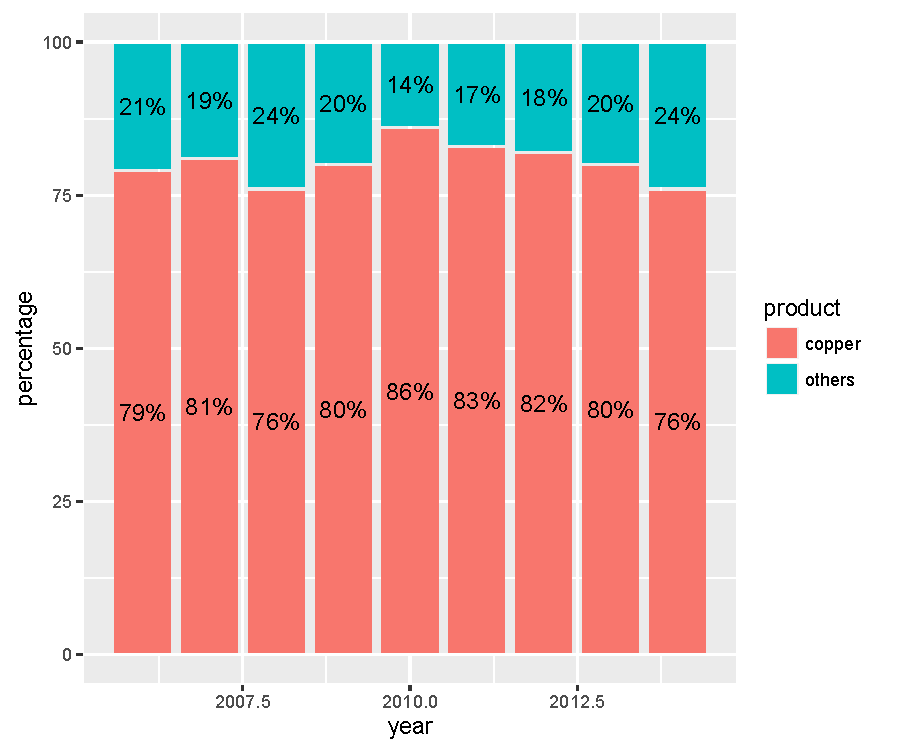
\includegraphics[width=0.6\linewidth]{4_Stacked_Bar_pdf/stacked_3-1} \end{center}

\section{Adjusting legend position}\label{adjusting-legend-position}

To adjust the position of the legend from the default spot of right of
the graph, we add the \texttt{theme} option and specify the
\texttt{legend.position="bottom"} argument. We can also change the title
to blank using the \texttt{legend.title\ =\ element\_blank()} argument
and change the legend shape using the\newline
\texttt{legend.direction="horizontal"} argument.

\begin{Shaded}
\begin{Highlighting}[]
\NormalTok{p4 <-}\StringTok{ }\NormalTok{p4 +}\StringTok{ }\KeywordTok{theme}\NormalTok{(}\DataTypeTok{legend.position=}\StringTok{"bottom"}\NormalTok{, }\DataTypeTok{legend.direction=}\StringTok{"horizontal"}\NormalTok{, }
  \DataTypeTok{legend.title =} \KeywordTok{element_blank}\NormalTok{())}
\NormalTok{p4}
\end{Highlighting}
\end{Shaded}

\begin{center}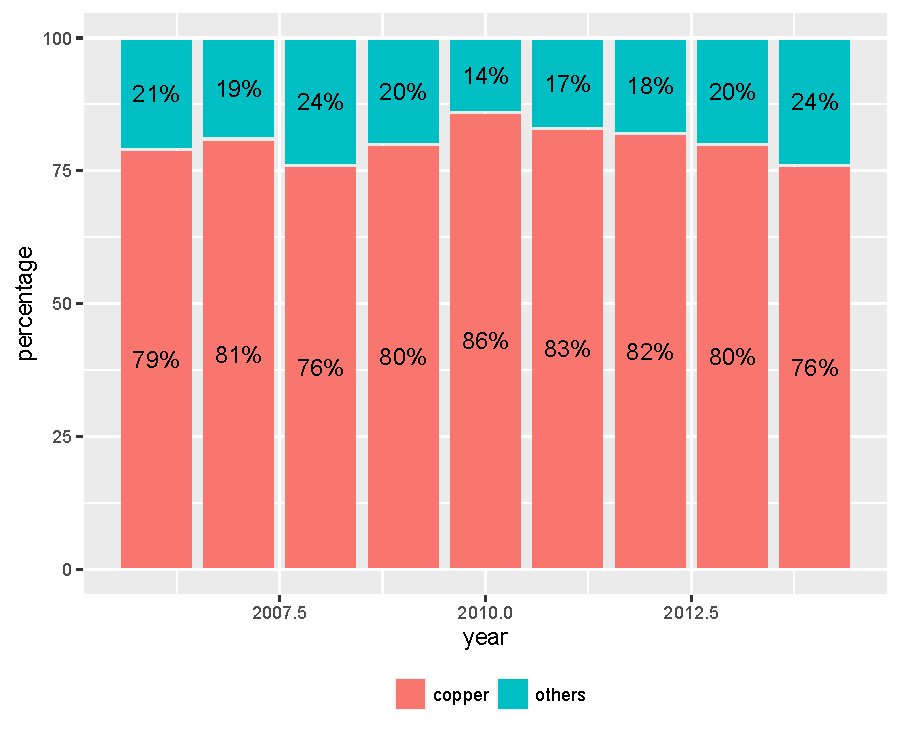
\includegraphics[width=0.6\linewidth]{4_Stacked_Bar_pdf/stacked_4-1} \end{center}

\section{Changing variables display}\label{changing-variables-display}

To change the variables' displayed name, we need to re-factor our data
labels in \texttt{charts.data} data frame.

\begin{Shaded}
\begin{Highlighting}[]
\NormalTok{charts.data <-}\StringTok{ }\KeywordTok{as.data.frame}\NormalTok{(charts.data)}
\NormalTok{charts.data$product <-}\StringTok{ }\KeywordTok{factor}\NormalTok{(charts.data$product, }\DataTypeTok{levels =} \KeywordTok{c}\NormalTok{(}\StringTok{"copper"}\NormalTok{,}\StringTok{"others"}\NormalTok{), }
  \DataTypeTok{labels =} \KeywordTok{c}\NormalTok{(}\StringTok{"Copper "}\NormalTok{,}\StringTok{"Pulp wood, Fruit, Salmon & Others"}\NormalTok{))}

\NormalTok{p4 <-}\StringTok{ }\KeywordTok{ggplot}\NormalTok{() +}\StringTok{ }
\StringTok{  }\KeywordTok{geom_bar}\NormalTok{(}\KeywordTok{aes}\NormalTok{(}\DataTypeTok{y =} \NormalTok{percentage, }\DataTypeTok{x =} \NormalTok{year, }\DataTypeTok{fill =} \NormalTok{product), }\DataTypeTok{data =} \NormalTok{charts.data, }
    \DataTypeTok{stat=}\StringTok{"identity"}\NormalTok{) +}\StringTok{ }
\StringTok{  }\KeywordTok{geom_text}\NormalTok{(}\DataTypeTok{data=}\NormalTok{charts.data, }\KeywordTok{aes}\NormalTok{(}\DataTypeTok{x =} \NormalTok{year, }\DataTypeTok{y =} \NormalTok{pos, }\DataTypeTok{label =} \KeywordTok{paste0}\NormalTok{(percentage,}\StringTok{"%"}\NormalTok{)), }
    \DataTypeTok{size=}\DecValTok{4}\NormalTok{) +}
\StringTok{  }\KeywordTok{theme}\NormalTok{(}\DataTypeTok{legend.position=}\StringTok{"bottom"}\NormalTok{, }\DataTypeTok{legend.direction=}\StringTok{"horizontal"}\NormalTok{, }\DataTypeTok{legend.title =} 
    \KeywordTok{element_blank}\NormalTok{())}
\NormalTok{p4}
\end{Highlighting}
\end{Shaded}

\begin{center}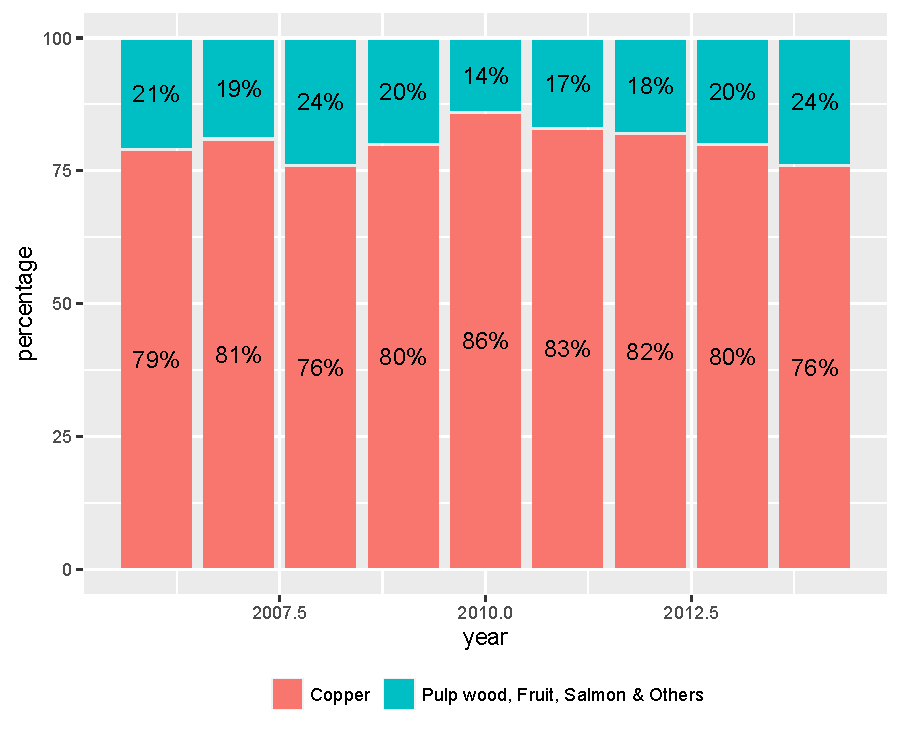
\includegraphics[width=0.6\linewidth]{4_Stacked_Bar_pdf/stacked_5-1} \end{center}

\section{Adjusting x-axis scale}\label{adjusting-x-axis-scale}

To change the axis tick marks, we use the \texttt{scale\_x\_continuous}
and/or \texttt{scale\_y\_continuous} commands.

\begin{Shaded}
\begin{Highlighting}[]
\NormalTok{p4 <-}\StringTok{ }\NormalTok{p4 +}\StringTok{ }\KeywordTok{scale_x_continuous}\NormalTok{(}\DataTypeTok{breaks=}\KeywordTok{seq}\NormalTok{(}\DecValTok{2006}\NormalTok{,}\DecValTok{2014}\NormalTok{,}\DecValTok{1}\NormalTok{))}
\NormalTok{p4}
\end{Highlighting}
\end{Shaded}

\begin{center}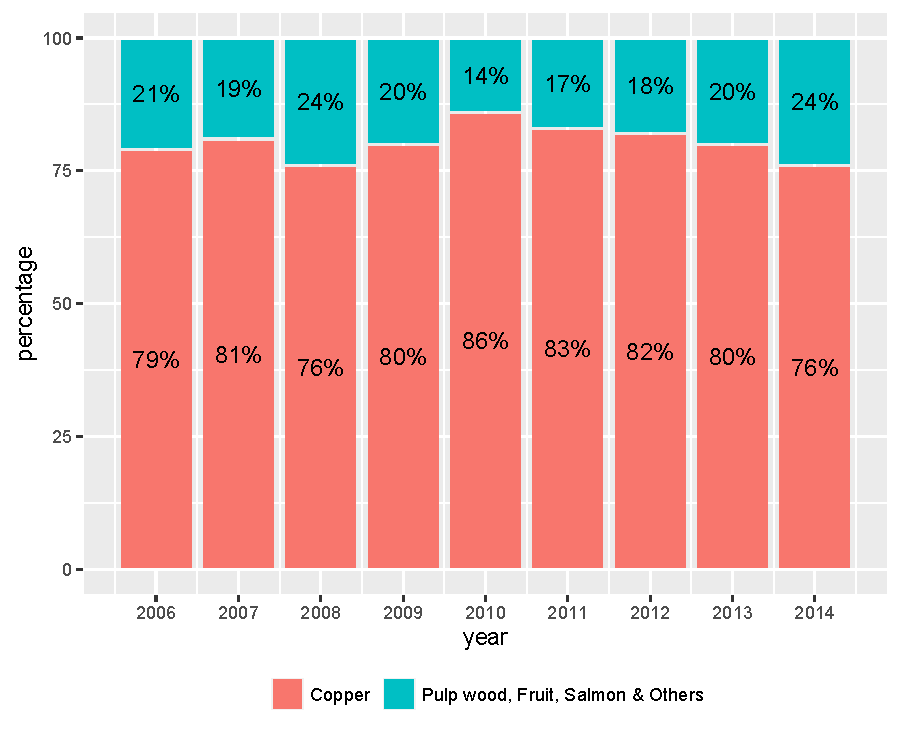
\includegraphics[width=0.6\linewidth]{4_Stacked_Bar_pdf/stacked_6-1} \end{center}

\section{Adjusting axis, title \&
units}\label{adjusting-axis-title-units}

To add a title, we include the option \texttt{ggtitle} and include the
name of the graph as a string argument, and to change the axis names we
use the \texttt{labs} command.

\begin{Shaded}
\begin{Highlighting}[]
\NormalTok{p4 <-}\StringTok{ }\NormalTok{p4 +}\StringTok{ }\KeywordTok{labs}\NormalTok{(}\DataTypeTok{x=}\StringTok{"Year"}\NormalTok{, }\DataTypeTok{y=}\StringTok{"Percentage"}\NormalTok{) +}\StringTok{ }
\StringTok{  }\KeywordTok{scale_y_continuous}\NormalTok{(}\DataTypeTok{labels =} \KeywordTok{dollar_format}\NormalTok{(}\DataTypeTok{suffix =} \StringTok{"%"}\NormalTok{, }\DataTypeTok{prefix =} \StringTok{""}\NormalTok{)) +}
\StringTok{  }\KeywordTok{ggtitle}\NormalTok{(}\StringTok{"Composition of Exports to China (%)"}\NormalTok{) }
\NormalTok{p4}
\end{Highlighting}
\end{Shaded}

\begin{center}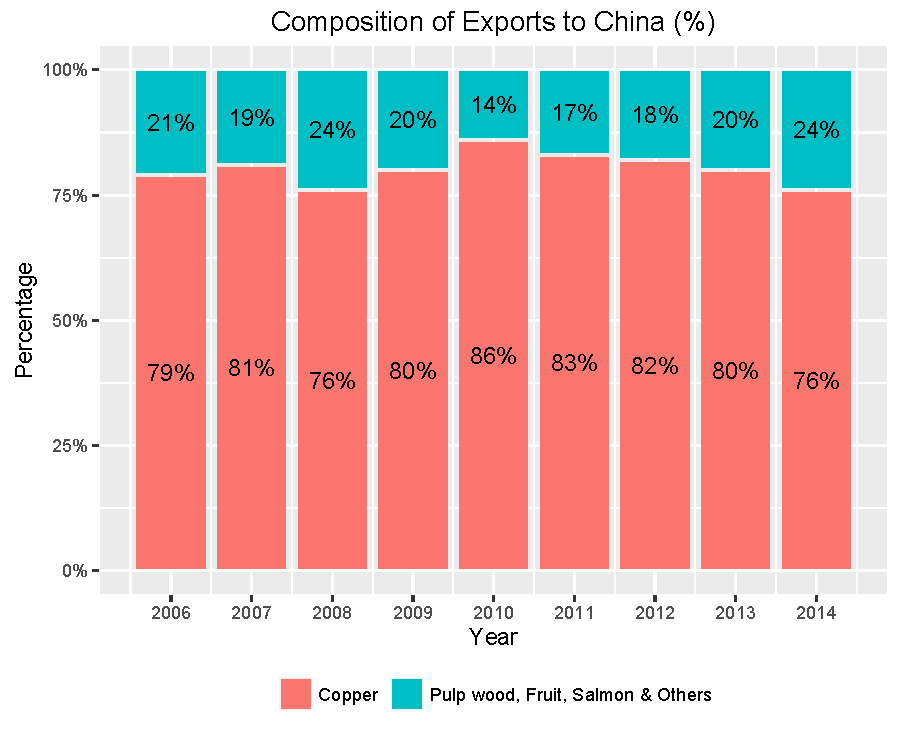
\includegraphics[width=0.6\linewidth]{4_Stacked_Bar_pdf/stacked_7-1} \end{center}

\section{Adjusting color palette}\label{adjusting-color-palette}

To change the colours, we use the \texttt{scale\_colour\_manual}
command. Note that you can reference the specific colours you'd like to
use with specific HEX codes. You can also reference colours by name,
with the full list of colours recognised by R
\href{http://www.stat.columbia.edu/~tzheng/files/Rcolor.pdf}{here}.

\begin{Shaded}
\begin{Highlighting}[]
\NormalTok{fill <-}\StringTok{ }\KeywordTok{c}\NormalTok{(}\StringTok{"#5F9EA0"}\NormalTok{, }\StringTok{"#E1B378"}\NormalTok{)}
\NormalTok{p4 <-}\StringTok{ }\NormalTok{p4 +}\StringTok{ }\KeywordTok{scale_fill_manual}\NormalTok{(}\DataTypeTok{values=}\NormalTok{fill)}
\NormalTok{p4}
\end{Highlighting}
\end{Shaded}

\begin{center}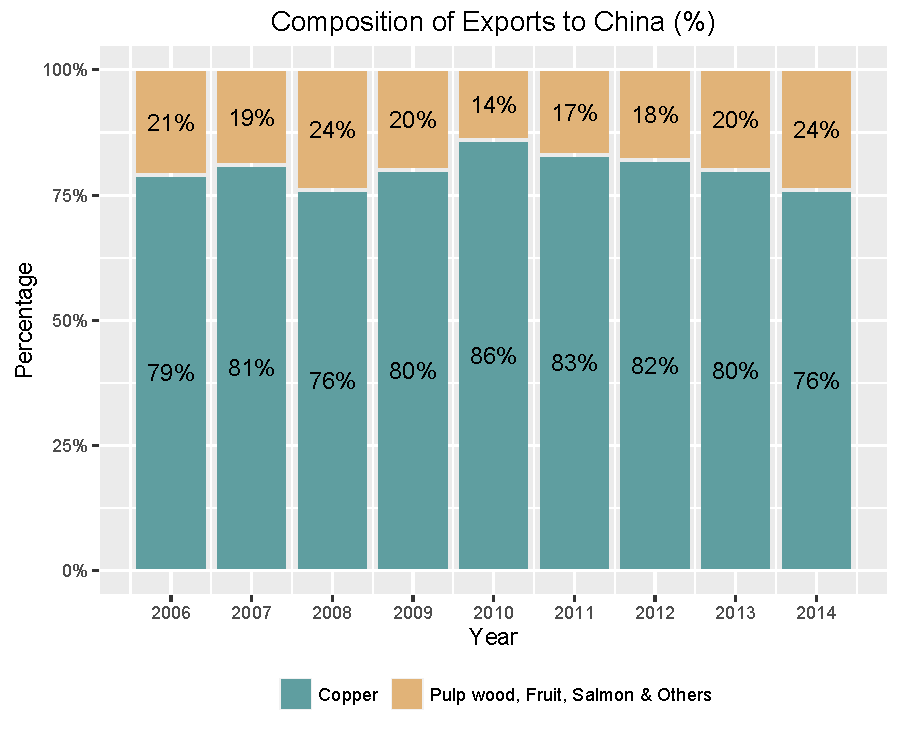
\includegraphics[width=0.6\linewidth]{4_Stacked_Bar_pdf/stacked_8-1} \end{center}

\section{Using the white theme}\label{using-the-white-theme}

As explained in the previous posts, we can also change the overall look
of the graph using themes. We'll start using a simple theme
customisation by adding \texttt{theme\_bw()} after \texttt{ggplot()}. As
you can see, we can further tweak the graph using the \texttt{theme}
option, which we've used so far to change the legend.

\begin{Shaded}
\begin{Highlighting}[]
\NormalTok{p4 <-}\StringTok{ }\KeywordTok{ggplot}\NormalTok{() +}\StringTok{ }
\StringTok{  }\KeywordTok{geom_bar}\NormalTok{(}\KeywordTok{aes}\NormalTok{(}\DataTypeTok{y =} \NormalTok{percentage, }\DataTypeTok{x =} \NormalTok{year, }\DataTypeTok{fill =} \NormalTok{product), }\DataTypeTok{data =} \NormalTok{charts.data, }
    \DataTypeTok{stat=}\StringTok{"identity"}\NormalTok{) +}\StringTok{ }
\StringTok{  }\KeywordTok{geom_text}\NormalTok{(}\DataTypeTok{data=}\NormalTok{charts.data, }\KeywordTok{aes}\NormalTok{(}\DataTypeTok{x =} \NormalTok{year, }\DataTypeTok{y =} \NormalTok{pos, }\DataTypeTok{label =} \KeywordTok{paste0}\NormalTok{(percentage,}\StringTok{"%"}\NormalTok{)), }
    \DataTypeTok{size=}\DecValTok{4}\NormalTok{) +}\StringTok{ }
\StringTok{  }\KeywordTok{scale_x_continuous}\NormalTok{(}\DataTypeTok{breaks=}\KeywordTok{seq}\NormalTok{(}\DecValTok{2006}\NormalTok{,}\DecValTok{2014}\NormalTok{,}\DecValTok{1}\NormalTok{)) +}\StringTok{ }
\StringTok{  }\KeywordTok{scale_y_continuous}\NormalTok{(}\DataTypeTok{labels =} \KeywordTok{dollar_format}\NormalTok{(}\DataTypeTok{suffix =} \StringTok{"%"}\NormalTok{, }\DataTypeTok{prefix =} \StringTok{""}\NormalTok{)) +}\StringTok{ }
\StringTok{  }\KeywordTok{labs}\NormalTok{(}\DataTypeTok{x=}\StringTok{"Year"}\NormalTok{, }\DataTypeTok{y=}\StringTok{"Percentage"}\NormalTok{) +}\StringTok{ }
\StringTok{  }\KeywordTok{ggtitle}\NormalTok{(}\StringTok{"Composition of Exports to China (%)"}\NormalTok{) +}
\StringTok{  }\KeywordTok{theme_bw}\NormalTok{() +}
\StringTok{  }\KeywordTok{theme}\NormalTok{(}\DataTypeTok{legend.position=}\StringTok{"bottom"}\NormalTok{, }
    \DataTypeTok{legend.direction=}\StringTok{"horizontal"}\NormalTok{, }
    \DataTypeTok{legend.title =} \KeywordTok{element_blank}\NormalTok{())    }
\NormalTok{p4}
\end{Highlighting}
\end{Shaded}

\begin{center}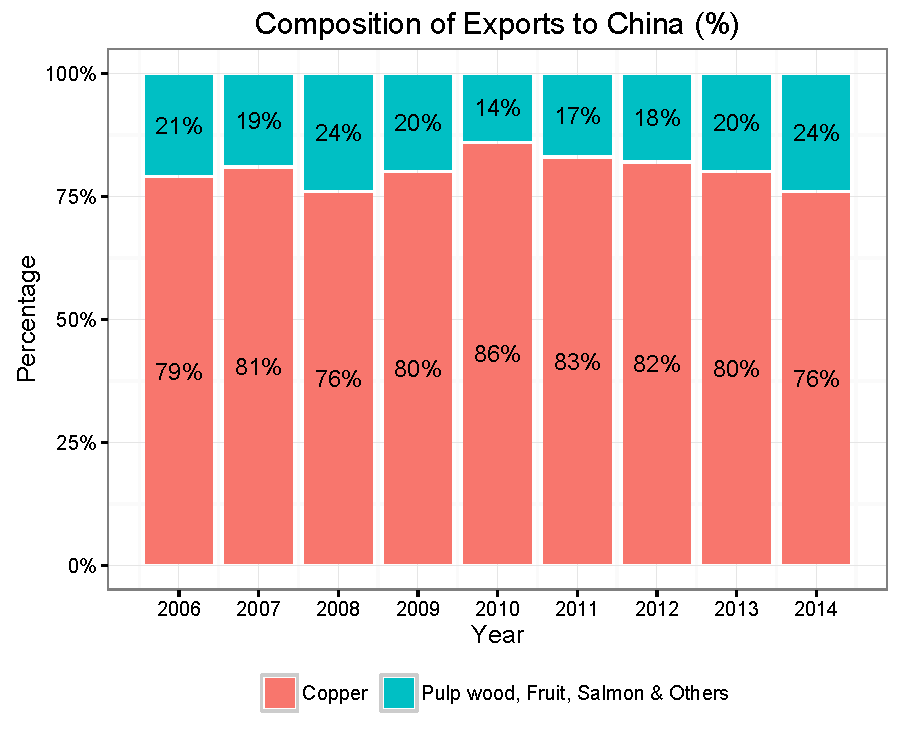
\includegraphics[width=0.6\linewidth]{4_Stacked_Bar_pdf/stacked_9-1} \end{center}

\section{Creating an XKCD style
chart}\label{creating-an-xkcd-style-chart}

Of course, you may want to create your own themes as well.
\texttt{ggplot2} allows for a very high degree of customisation,
including allowing you to use imported fonts. Below is an example of a
theme Mauricio was able to create which mimics the visual style of
\href{http://xkcd.com/}{XKCD}. In order to create this chart, you first
need to import the XKCD font, and load it into R using the
\texttt{extrafont} package.

\begin{Shaded}
\begin{Highlighting}[]
\NormalTok{fill <-}\StringTok{ }\KeywordTok{c}\NormalTok{(}\StringTok{"#40b8d0"}\NormalTok{, }\StringTok{"#b2d183"}\NormalTok{)}

\NormalTok{p4 <-}\StringTok{ }\KeywordTok{ggplot}\NormalTok{() +}\StringTok{ }
\StringTok{  }\KeywordTok{geom_bar}\NormalTok{(}\KeywordTok{aes}\NormalTok{(}\DataTypeTok{y =} \NormalTok{percentage, }\DataTypeTok{x =} \NormalTok{year, }\DataTypeTok{fill =} \NormalTok{product), }\DataTypeTok{data =} \NormalTok{charts.data, }
    \DataTypeTok{stat=}\StringTok{"identity"}\NormalTok{) +}\StringTok{ }
\StringTok{  }\KeywordTok{geom_text}\NormalTok{(}\DataTypeTok{data=}\NormalTok{charts.data, }\KeywordTok{aes}\NormalTok{(}\DataTypeTok{x =} \NormalTok{year, }\DataTypeTok{y =} \NormalTok{pos, }\DataTypeTok{label =} \KeywordTok{paste0}\NormalTok{(percentage,}\StringTok{"%"}\NormalTok{)), }
    \DataTypeTok{colour=}\StringTok{"black"}\NormalTok{, }\DataTypeTok{family=}\StringTok{"xkcd-Regular"}\NormalTok{, }\DataTypeTok{size =} \DecValTok{5}\NormalTok{, }\DataTypeTok{show.legend =} \NormalTok{F) +}\StringTok{ }
\StringTok{  }\KeywordTok{scale_x_continuous}\NormalTok{(}\DataTypeTok{breaks=}\KeywordTok{seq}\NormalTok{(}\DecValTok{2006}\NormalTok{,}\DecValTok{2014}\NormalTok{,}\DecValTok{1}\NormalTok{)) +}\StringTok{ }
\StringTok{  }\KeywordTok{scale_y_continuous}\NormalTok{(}\DataTypeTok{labels =} \KeywordTok{dollar_format}\NormalTok{(}\DataTypeTok{suffix =} \StringTok{"%"}\NormalTok{, }\DataTypeTok{prefix =} \StringTok{""}\NormalTok{)) +}\StringTok{ }
\StringTok{  }\KeywordTok{labs}\NormalTok{(}\DataTypeTok{x=}\StringTok{"Year"}\NormalTok{, }\DataTypeTok{y=}\StringTok{"Percentage"}\NormalTok{) +}\StringTok{ }
\StringTok{  }\KeywordTok{ggtitle}\NormalTok{(}\StringTok{"Composition of Exports to China (%)"}\NormalTok{) +}\StringTok{ }
\StringTok{  }\KeywordTok{scale_fill_manual}\NormalTok{(}\DataTypeTok{values=}\NormalTok{fill) +}\StringTok{ }
\StringTok{  }\KeywordTok{theme}\NormalTok{(}\DataTypeTok{axis.line.x =} \KeywordTok{element_line}\NormalTok{(}\DataTypeTok{size=}\NormalTok{.}\DecValTok{5}\NormalTok{, }\DataTypeTok{colour =} \StringTok{"black"}\NormalTok{), }
    \DataTypeTok{axis.line.y =} \KeywordTok{element_line}\NormalTok{(}\DataTypeTok{size=}\NormalTok{.}\DecValTok{5}\NormalTok{, }\DataTypeTok{colour =} \StringTok{"black"}\NormalTok{),}
    \DataTypeTok{axis.text.x=}\KeywordTok{element_text}\NormalTok{(}\DataTypeTok{colour=}\StringTok{"black"}\NormalTok{, }\DataTypeTok{size =} \DecValTok{10}\NormalTok{), }
    \DataTypeTok{axis.text.y=}\KeywordTok{element_text}\NormalTok{(}\DataTypeTok{colour=}\StringTok{"black"}\NormalTok{, }\DataTypeTok{size =} \DecValTok{10}\NormalTok{),}
    \DataTypeTok{axis.line.x =} \KeywordTok{element_line}\NormalTok{(}\DataTypeTok{size=}\NormalTok{.}\DecValTok{5}\NormalTok{, }\DataTypeTok{colour =} \StringTok{"black"}\NormalTok{),}
    \DataTypeTok{legend.key=}\KeywordTok{element_rect}\NormalTok{(}\DataTypeTok{fill=}\StringTok{"white"}\NormalTok{, }\DataTypeTok{colour=}\StringTok{"white"}\NormalTok{),}
    \DataTypeTok{legend.position=}\StringTok{"bottom"}\NormalTok{, }\DataTypeTok{legend.direction=}\StringTok{"horizontal"}\NormalTok{, }
    \DataTypeTok{legend.title =} \KeywordTok{element_blank}\NormalTok{(),}
    \DataTypeTok{panel.grid.major =} \KeywordTok{element_blank}\NormalTok{(),}
    \DataTypeTok{panel.grid.minor =} \KeywordTok{element_blank}\NormalTok{(), }\DataTypeTok{panel.border =} \KeywordTok{element_blank}\NormalTok{(), }
    \DataTypeTok{panel.background =} \KeywordTok{element_blank}\NormalTok{(),}
    \DataTypeTok{plot.title=}\KeywordTok{element_text}\NormalTok{(}\DataTypeTok{family=}\StringTok{"xkcd-Regular"}\NormalTok{), }
    \DataTypeTok{text=}\KeywordTok{element_text}\NormalTok{(}\DataTypeTok{family=}\StringTok{"xkcd-Regular"}\NormalTok{)) }
\NormalTok{p4}
\end{Highlighting}
\end{Shaded}

\begin{center}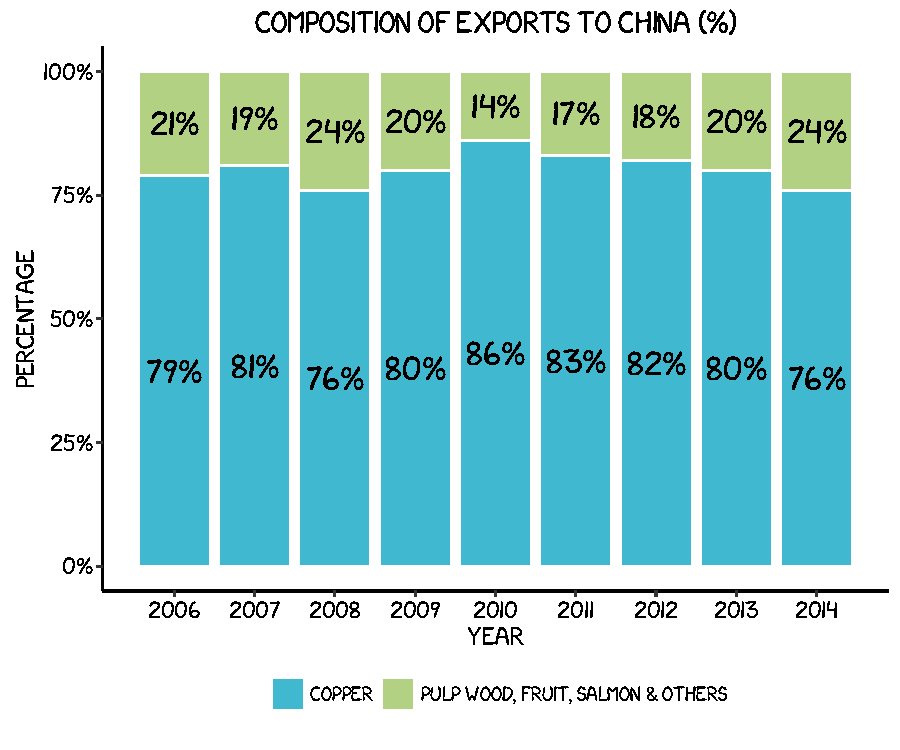
\includegraphics[width=0.6\linewidth]{4_Stacked_Bar_pdf/stacked_10-1} \end{center}

\section{\texorpdfstring{Using `The Economist'
theme}{Using The Economist theme}}\label{using-the-economist-theme}

There are a wider range of pre-built themes available as part of the
\texttt{ggthemes} package (more information on these
\href{https://cran.r-project.org/web/packages/ggthemes/vignettes/ggthemes.html}{here}).
Below we've applied \texttt{theme\_economist()}, which approximates
graphs in the Economist magazine. It is also important that the font
change argument inside \texttt{theme} is optional and it's only to
obtain a more similar result compared to the original. For an exact
result you need `Officina Sans' which is a commercial font and is
available \href{http://www.myfonts.com/fonts/itc/officina-sans/}{here}.

\begin{Shaded}
\begin{Highlighting}[]
\NormalTok{p4 <-}\StringTok{ }\KeywordTok{ggplot}\NormalTok{() +}
\StringTok{  }\KeywordTok{geom_bar}\NormalTok{(}\KeywordTok{aes}\NormalTok{(}\DataTypeTok{y =} \NormalTok{percentage, }\DataTypeTok{x =} \NormalTok{year, }\DataTypeTok{fill =} \NormalTok{product), }\DataTypeTok{data =} \NormalTok{charts.data, }
    \DataTypeTok{stat=}\StringTok{"identity"}\NormalTok{) +}\StringTok{ }
\StringTok{  }\KeywordTok{geom_text}\NormalTok{(}\DataTypeTok{data=}\NormalTok{charts.data, }\KeywordTok{aes}\NormalTok{(}\DataTypeTok{x =} \NormalTok{year, }\DataTypeTok{y =} \NormalTok{pos, }\DataTypeTok{label =} \KeywordTok{paste0}\NormalTok{(percentage,}\StringTok{"%"}\NormalTok{)), }
    \DataTypeTok{colour=}\StringTok{"white"}\NormalTok{, }\DataTypeTok{family=}\StringTok{"OfficinaSanITC-Book"}\NormalTok{, }\DataTypeTok{size=}\DecValTok{4}\NormalTok{) +}\StringTok{ }
\StringTok{  }\KeywordTok{scale_x_continuous}\NormalTok{(}\DataTypeTok{breaks=}\KeywordTok{seq}\NormalTok{(}\DecValTok{2006}\NormalTok{,}\DecValTok{2014}\NormalTok{,}\DecValTok{1}\NormalTok{)) +}\StringTok{ }
\StringTok{  }\KeywordTok{scale_y_continuous}\NormalTok{(}\DataTypeTok{labels =} \KeywordTok{dollar_format}\NormalTok{(}\DataTypeTok{suffix =} \StringTok{"%"}\NormalTok{, }\DataTypeTok{prefix =} \StringTok{""}\NormalTok{)) +}\StringTok{ }
\StringTok{  }\KeywordTok{labs}\NormalTok{(}\DataTypeTok{x=}\StringTok{"Year"}\NormalTok{, }\DataTypeTok{y=}\StringTok{"Percentage"}\NormalTok{) +}\StringTok{ }
\StringTok{  }\KeywordTok{ggtitle}\NormalTok{(}\StringTok{"Composition of Exports to China (%)"}\NormalTok{) +}
\StringTok{  }\KeywordTok{theme_economist}\NormalTok{() +}\StringTok{ }\KeywordTok{scale_fill_economist}\NormalTok{() +}\StringTok{ }
\StringTok{  }\KeywordTok{theme}\NormalTok{(}\DataTypeTok{axis.line.x =} \KeywordTok{element_line}\NormalTok{(}\DataTypeTok{size=}\NormalTok{.}\DecValTok{5}\NormalTok{, }\DataTypeTok{colour =} \StringTok{"black"}\NormalTok{),}
    \DataTypeTok{legend.position=}\StringTok{"bottom"}\NormalTok{, }
    \DataTypeTok{legend.direction=}\StringTok{"horizontal"}\NormalTok{, }
    \DataTypeTok{legend.title =} \KeywordTok{element_blank}\NormalTok{(),}
    \DataTypeTok{plot.title=}\KeywordTok{element_text}\NormalTok{(}\DataTypeTok{family=}\StringTok{"OfficinaSanITC-Book"}\NormalTok{),}
    \DataTypeTok{text=}\KeywordTok{element_text}\NormalTok{(}\DataTypeTok{family=}\StringTok{"OfficinaSanITC-Book"}\NormalTok{))    }
\NormalTok{p4}
\end{Highlighting}
\end{Shaded}

\begin{center}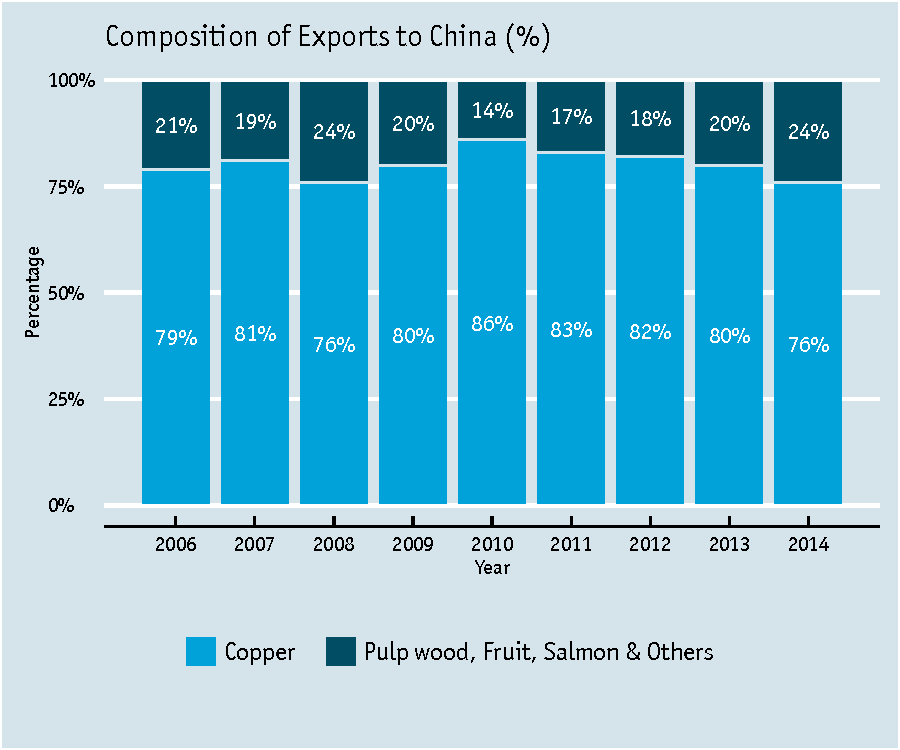
\includegraphics[width=0.6\linewidth]{4_Stacked_Bar_pdf/stacked_11-1} \end{center}

\section{\texorpdfstring{Using `Five Thirty Eight'
theme}{Using Five Thirty Eight theme}}\label{using-five-thirty-eight-theme}

Below we've applied \texttt{theme\_fivethirtyeight()}, which
approximates graphs in the nice
\href{http://fivethirtyeight.com/}{FiveThirtyEight} website. Again, it
is also important that the font change is optional and it's only to
obtain a more similar result compared to the original. For an exact
result you need `Atlas Grotesk' and `Decima Mono Pro' which are
commercial font and are available
\href{https://commercialtype.com/catalog/atlas}{here} and
\href{https://www.myfonts.com/fonts/tipografiaramis/decima-mono-pro/}{here}.

\begin{Shaded}
\begin{Highlighting}[]
\NormalTok{p4 <-}\StringTok{ }\KeywordTok{ggplot}\NormalTok{() +}
\StringTok{  }\KeywordTok{geom_bar}\NormalTok{(}\KeywordTok{aes}\NormalTok{(}\DataTypeTok{y =} \NormalTok{percentage, }\DataTypeTok{x =} \NormalTok{year, }\DataTypeTok{fill =} \NormalTok{product), }\DataTypeTok{data =} \NormalTok{charts.data, }
    \DataTypeTok{stat=}\StringTok{"identity"}\NormalTok{) +}\StringTok{ }
\StringTok{  }\KeywordTok{geom_text}\NormalTok{(}\DataTypeTok{data=}\NormalTok{charts.data, }\KeywordTok{aes}\NormalTok{(}\DataTypeTok{x =} \NormalTok{year, }\DataTypeTok{y =} \NormalTok{pos, }\DataTypeTok{label =} \KeywordTok{paste0}\NormalTok{(percentage,}\StringTok{"%"}\NormalTok{)), }
    \DataTypeTok{colour=}\StringTok{"white"}\NormalTok{, }\DataTypeTok{family=}\StringTok{"DecimaMonoPro-Bold"}\NormalTok{, }\DataTypeTok{size=}\DecValTok{4}\NormalTok{) +}\StringTok{ }
\StringTok{  }\KeywordTok{scale_x_continuous}\NormalTok{(}\DataTypeTok{breaks=}\KeywordTok{seq}\NormalTok{(}\DecValTok{2006}\NormalTok{,}\DecValTok{2014}\NormalTok{,}\DecValTok{1}\NormalTok{)) +}\StringTok{ }
\StringTok{  }\KeywordTok{scale_y_continuous}\NormalTok{(}\DataTypeTok{labels =} \KeywordTok{dollar_format}\NormalTok{(}\DataTypeTok{suffix =} \StringTok{"%"}\NormalTok{, }\DataTypeTok{prefix =} \StringTok{""}\NormalTok{)) +}\StringTok{ }
\StringTok{  }\KeywordTok{labs}\NormalTok{(}\DataTypeTok{x=}\StringTok{"Year"}\NormalTok{, }\DataTypeTok{y=}\StringTok{"Percentage"}\NormalTok{) +}\StringTok{ }
\StringTok{  }\KeywordTok{ggtitle}\NormalTok{(}\StringTok{"Composition of Exports to China (%)"}\NormalTok{) +}
\StringTok{  }\KeywordTok{theme_fivethirtyeight}\NormalTok{() +}\StringTok{ }\KeywordTok{scale_fill_fivethirtyeight}\NormalTok{() +}\StringTok{   }
\StringTok{  }\KeywordTok{theme}\NormalTok{(}\DataTypeTok{axis.title =} \KeywordTok{element_text}\NormalTok{(}\DataTypeTok{family=}\StringTok{"Atlas Grotesk Regular"}\NormalTok{),}
    \DataTypeTok{legend.position=}\StringTok{"bottom"}\NormalTok{, }\DataTypeTok{legend.direction=}\StringTok{"horizontal"}\NormalTok{, }
    \DataTypeTok{legend.title=}\KeywordTok{element_blank}\NormalTok{(),}
    \DataTypeTok{plot.title=}\KeywordTok{element_text}\NormalTok{(}\DataTypeTok{family=}\StringTok{"Atlas Grotesk Medium"}\NormalTok{), }
    \DataTypeTok{legend.text=}\KeywordTok{element_text}\NormalTok{(}\DataTypeTok{family=}\StringTok{"Atlas Grotesk Regular"}\NormalTok{),}
    \DataTypeTok{text=}\KeywordTok{element_text}\NormalTok{(}\DataTypeTok{family=}\StringTok{"DecimaMonoPro"}\NormalTok{)) }
\NormalTok{p4}
\end{Highlighting}
\end{Shaded}

\begin{center}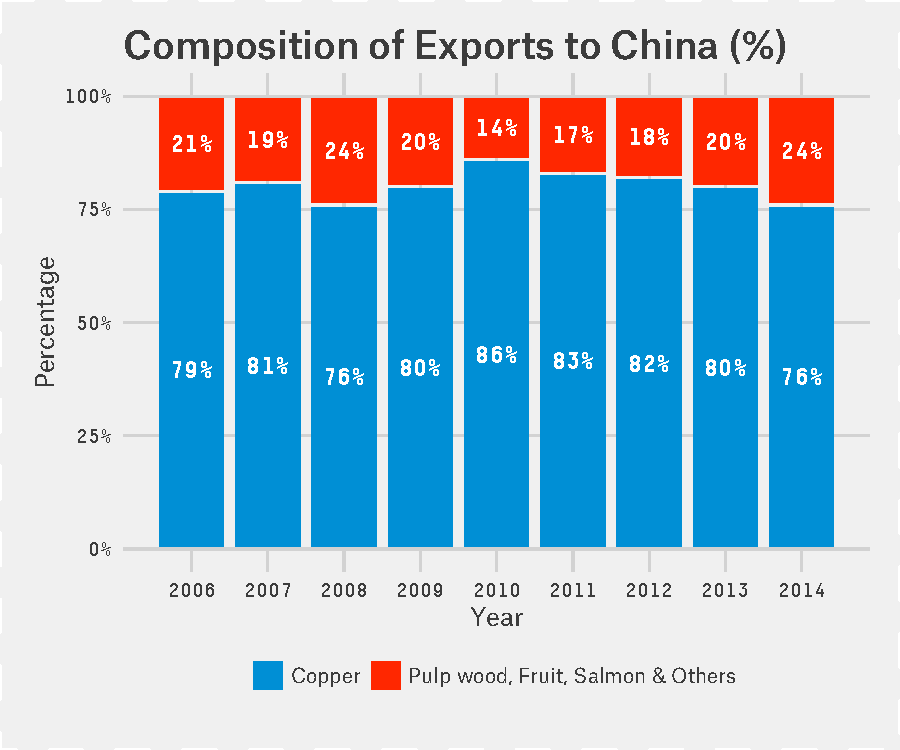
\includegraphics[width=0.6\linewidth]{4_Stacked_Bar_pdf/stacked_12-1} \end{center}

\section{Creating your own theme}\label{creating-your-own-theme}

As before, you can modify your plots a lot as \texttt{ggplot2} allows
many customisations. Here we present our original result shown at the
top of page.

\begin{Shaded}
\begin{Highlighting}[]
\NormalTok{fill <-}\StringTok{ }\KeywordTok{c}\NormalTok{(}\StringTok{"#40b8d0"}\NormalTok{, }\StringTok{"#b2d183"}\NormalTok{)}

\NormalTok{p4 <-}\StringTok{ }\KeywordTok{ggplot}\NormalTok{() +}\StringTok{ }
\StringTok{  }\KeywordTok{geom_bar}\NormalTok{(}\KeywordTok{aes}\NormalTok{(}\DataTypeTok{y =} \NormalTok{percentage, }\DataTypeTok{x =} \NormalTok{year, }\DataTypeTok{fill =} \NormalTok{product), }\DataTypeTok{data =} \NormalTok{charts.data, }
    \DataTypeTok{stat=}\StringTok{"identity"}\NormalTok{) +}\StringTok{ }
\StringTok{  }\KeywordTok{geom_text}\NormalTok{(}\DataTypeTok{data=}\NormalTok{charts.data, }\KeywordTok{aes}\NormalTok{(}\DataTypeTok{x =} \NormalTok{year, }\DataTypeTok{y =} \NormalTok{pos, }\DataTypeTok{label =} \KeywordTok{paste0}\NormalTok{(percentage,}\StringTok{"%"}\NormalTok{)), }
    \DataTypeTok{colour=}\StringTok{"black"}\NormalTok{, }\DataTypeTok{family=}\StringTok{"Tahoma"}\NormalTok{, }\DataTypeTok{size=}\DecValTok{4}\NormalTok{) +}\StringTok{ }
\StringTok{  }\KeywordTok{scale_x_continuous}\NormalTok{(}\DataTypeTok{breaks=}\KeywordTok{seq}\NormalTok{(}\DecValTok{2006}\NormalTok{,}\DecValTok{2014}\NormalTok{,}\DecValTok{1}\NormalTok{)) +}\StringTok{ }
\StringTok{  }\KeywordTok{scale_y_continuous}\NormalTok{(}\DataTypeTok{labels =} \KeywordTok{dollar_format}\NormalTok{(}\DataTypeTok{suffix =} \StringTok{"%"}\NormalTok{, }\DataTypeTok{prefix =} \StringTok{""}\NormalTok{)) +}\StringTok{ }
\StringTok{  }\KeywordTok{labs}\NormalTok{(}\DataTypeTok{x=}\StringTok{"Year"}\NormalTok{, }\DataTypeTok{y=}\StringTok{"Percentage"}\NormalTok{) +}\StringTok{ }
\StringTok{  }\KeywordTok{ggtitle}\NormalTok{(}\StringTok{"Composition of Exports to China (%)"}\NormalTok{) +}\StringTok{ }
\StringTok{  }\KeywordTok{scale_fill_manual}\NormalTok{(}\DataTypeTok{values=}\NormalTok{fill) +}\StringTok{ }
\StringTok{  }\KeywordTok{theme}\NormalTok{(}\DataTypeTok{panel.border =} \KeywordTok{element_rect}\NormalTok{(}\DataTypeTok{colour =} \StringTok{"black"}\NormalTok{, }\DataTypeTok{fill=}\OtherTok{NA}\NormalTok{, }\DataTypeTok{size=}\NormalTok{.}\DecValTok{5}\NormalTok{),}
    \DataTypeTok{axis.text.x=}\KeywordTok{element_text}\NormalTok{(}\DataTypeTok{colour=}\StringTok{"black"}\NormalTok{, }\DataTypeTok{size =} \DecValTok{10}\NormalTok{), }
    \DataTypeTok{axis.text.y=}\KeywordTok{element_text}\NormalTok{(}\DataTypeTok{colour=}\StringTok{"black"}\NormalTok{, }\DataTypeTok{size =} \DecValTok{10}\NormalTok{),}
    \DataTypeTok{legend.key=}\KeywordTok{element_rect}\NormalTok{(}\DataTypeTok{fill=}\StringTok{"white"}\NormalTok{, }\DataTypeTok{colour=}\StringTok{"white"}\NormalTok{),}
    \DataTypeTok{legend.position=}\StringTok{"bottom"}\NormalTok{, }\DataTypeTok{legend.direction=}\StringTok{"horizontal"}\NormalTok{, }
    \DataTypeTok{legend.title =} \KeywordTok{element_blank}\NormalTok{(),}
    \DataTypeTok{panel.grid.major =} \KeywordTok{element_line}\NormalTok{(}\DataTypeTok{colour =} \StringTok{"#d3d3d3"}\NormalTok{), }
    \DataTypeTok{panel.grid.minor =} \KeywordTok{element_blank}\NormalTok{(), }
    \DataTypeTok{panel.border =} \KeywordTok{element_blank}\NormalTok{(), }
    \DataTypeTok{panel.background =} \KeywordTok{element_blank}\NormalTok{(),}
    \DataTypeTok{plot.title =} \KeywordTok{element_text}\NormalTok{(}\DataTypeTok{size =} \DecValTok{14}\NormalTok{, }\DataTypeTok{family =} \StringTok{"Tahoma"}\NormalTok{, }\DataTypeTok{face =} \StringTok{"bold"}\NormalTok{), }
    \DataTypeTok{text=}\KeywordTok{element_text}\NormalTok{(}\DataTypeTok{family=}\StringTok{"Tahoma"}\NormalTok{)) }
\NormalTok{p4}
\end{Highlighting}
\end{Shaded}

\begin{center}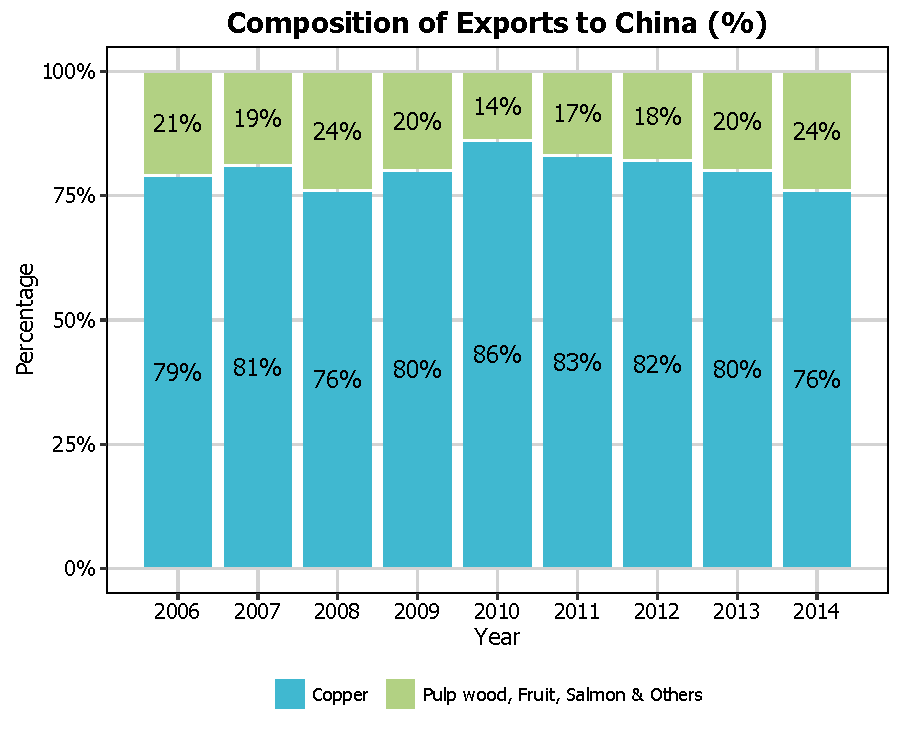
\includegraphics[width=0.6\linewidth]{4_Stacked_Bar_pdf/stacked_13-1} \end{center}
